\documentclass[12pt]{article}
\usepackage{amsmath, amssymb, graphicx}
\usepackage{geometry}
\usepackage{enumitem}
\geometry{a4paper, margin=1in}

\begin{document}

\title{Homework 2}
\author{Hao Yin}
\date{\today}
\maketitle

\section*{Question 1}
    \begin{enumerate}[label=\roman*.]
        \item (a)
        \[G(s) = \frac{4s-8}{s^2+2s-9}\]
        \[\text{DC GAIN} = G(0) = \frac{-8}{-9}\]

        (b)
        \[G(s) = \frac{10}{s^2+2s+10}\]
        \[\text{DC GAIN} = G(0) = \frac{10}{10} = 1\]

        \item (a)
        \[N(0) = s^2+2s-9 = 0\]
        \[\text{Poles:} s = -1 \pm \sqrt{10}\]
        \[Real(s) = -1 + \sqrt{10} > 0, \text{so this system is unstable.}\]

        (b)
        \[N(0) = s^2+2s+10 = 0\]
        \[\text{Poles:} s = -1 \pm 3i\]
        \[Real(s) = -1 < 0, \text{so this system is stable.}\]

        \item (a)
        
        From TF, we get the ODE:
        \[\ddot{y(t)} + 2\dot{y(t)} - 9y(t) = 4\dot{u(t)} - 8u(t)\]
        Guess that: $y(t) = Ce^{st}, \dot{y(t)} = Cse^{st}, 
            \ddot{y(t)} = Cs^2e^{st}$
        So we get:
        \[Cs^2e^{st} + 2Cse^{st} - 9Ce^{st} = 0\]
        \[Ce^{st} (s^2 + 2s - 9) = 0\]
        \[s = -1 \pm \sqrt{10}\]
        \[y(t) = c_1e^{(-1+\sqrt{10})t} + c_2e^{(-1-\sqrt{10})t}\]

        (b)

        From TF, we get the ODE:
        \[\ddot{y(t)} + 2\dot{y(t)} + 10y(t) = 10u(t)\]
        Guess that: $y(t) = Ce^{st}, \dot{y(t)} = Cse^{st}, 
            \ddot{y(t)} = Cs^2e^{st}$
        So we get:
        \[Cs^2e^{st} + 2Cse^{st} + 10Ce^{st} = 0\]
        \[Ce^{st} (s^2 + 2s + 10) = 0\]
        \[s = -1 \pm 3i\]
        \[y(t) = c_1e^{-t}cos(3t) + c_2e^{-t}sin(3t)\]

        \item (a)
        Roots: $s = -1 \pm \sqrt{10}$

        Homogeneous Solution: 
        \[y_h(t) = c_1e^{(-1+\sqrt{10})t} + c_2e^{(-1-\sqrt{10})t}\]

        Input: $u(t) \equiv 2$

        \[\ddot{y_p(t)} + 2\dot{y_p(t)} - 9y_p(t) = -16\]

        Guess $y_p(t) = C$ , need: $-9C = -16$ ,and then get: $C = \frac{16}{9}$

        So general form of Input response:

        \[y(t) = y_h(t) + y_p(t) = c_1e^{(-1+\sqrt{10})t} + c_2e^{(-1-\sqrt{10})t} + 
            \frac{16}{9}\]

        (b)
        Roots: $s = -1 \pm 3i$

        Homogeneous Solution: 
        \[y(t) = c_1e^{-t}cos(3t) + c_2e^{-t}sin(3t)\]

        Input: $u(t) \equiv 2$

        \[\ddot{y(t)} + 2\dot{y(t)} + 10y(t) = 20\]

        Guess $y_p(t) = C$ , need: $10C = 20$ ,and then get: $C = 2$

        So general form of Input response:

        \[y(t) = y_h(t) + y_p(t) = c_1e^{-t}cos(3t) + c_2e^{-t}sin(3t) + 2\]

        \item (a)
        For the zero initial conditions: $y(0) = 0, \dot{y(0)} = 0$

        We get:
        \[y(0) = c_1 + c_2 + \frac{16}{9} = 0\]
        \[\dot{y(0)} = (-1+\sqrt{10})c_1 + (-1-\sqrt{10}c_2) = 0\]

        So:
        \[c_1 = -1.17, c_2 = -0.6078\]

        So input response:
        \[y(t) = -1.17e^{(-1+\sqrt{10})t} -0.6078e^{(-1-\sqrt{10})t} + 
            \frac{16}{9}\]


        (b)
        For the zero initial conditions: $y(0) = 0, \dot{y(0)} = 0$

        We get:
        \[y(0) = c_1 + 2 = 0\]
        \[\dot{y(0)} = -c_1 + 3c_2 = 0\]

        So:
        \[c_1 = -2, c_2 = -2/3\]

        So input response:
        \[y(t) = -2e^{-t}cos(3t) - \frac{2}{3}e^{-t}sin(3t) + 2\]


    \end{enumerate}

\section*{Question 2}
    \begin{enumerate}[label=\alph*]
        \item TF:
        \[G(s) = \frac{4}{s+3}\]
        \[\text{Roots: } s = -3 < 0 \text{So this system is stable.}\]
        
        \item Poles: $s = -3$
        \[\text{Time constant: } \tau = \frac{1}{|Re(p)|} = \frac{1}{3}s\]

        \item y(0) = 0:
        \begin{center}
            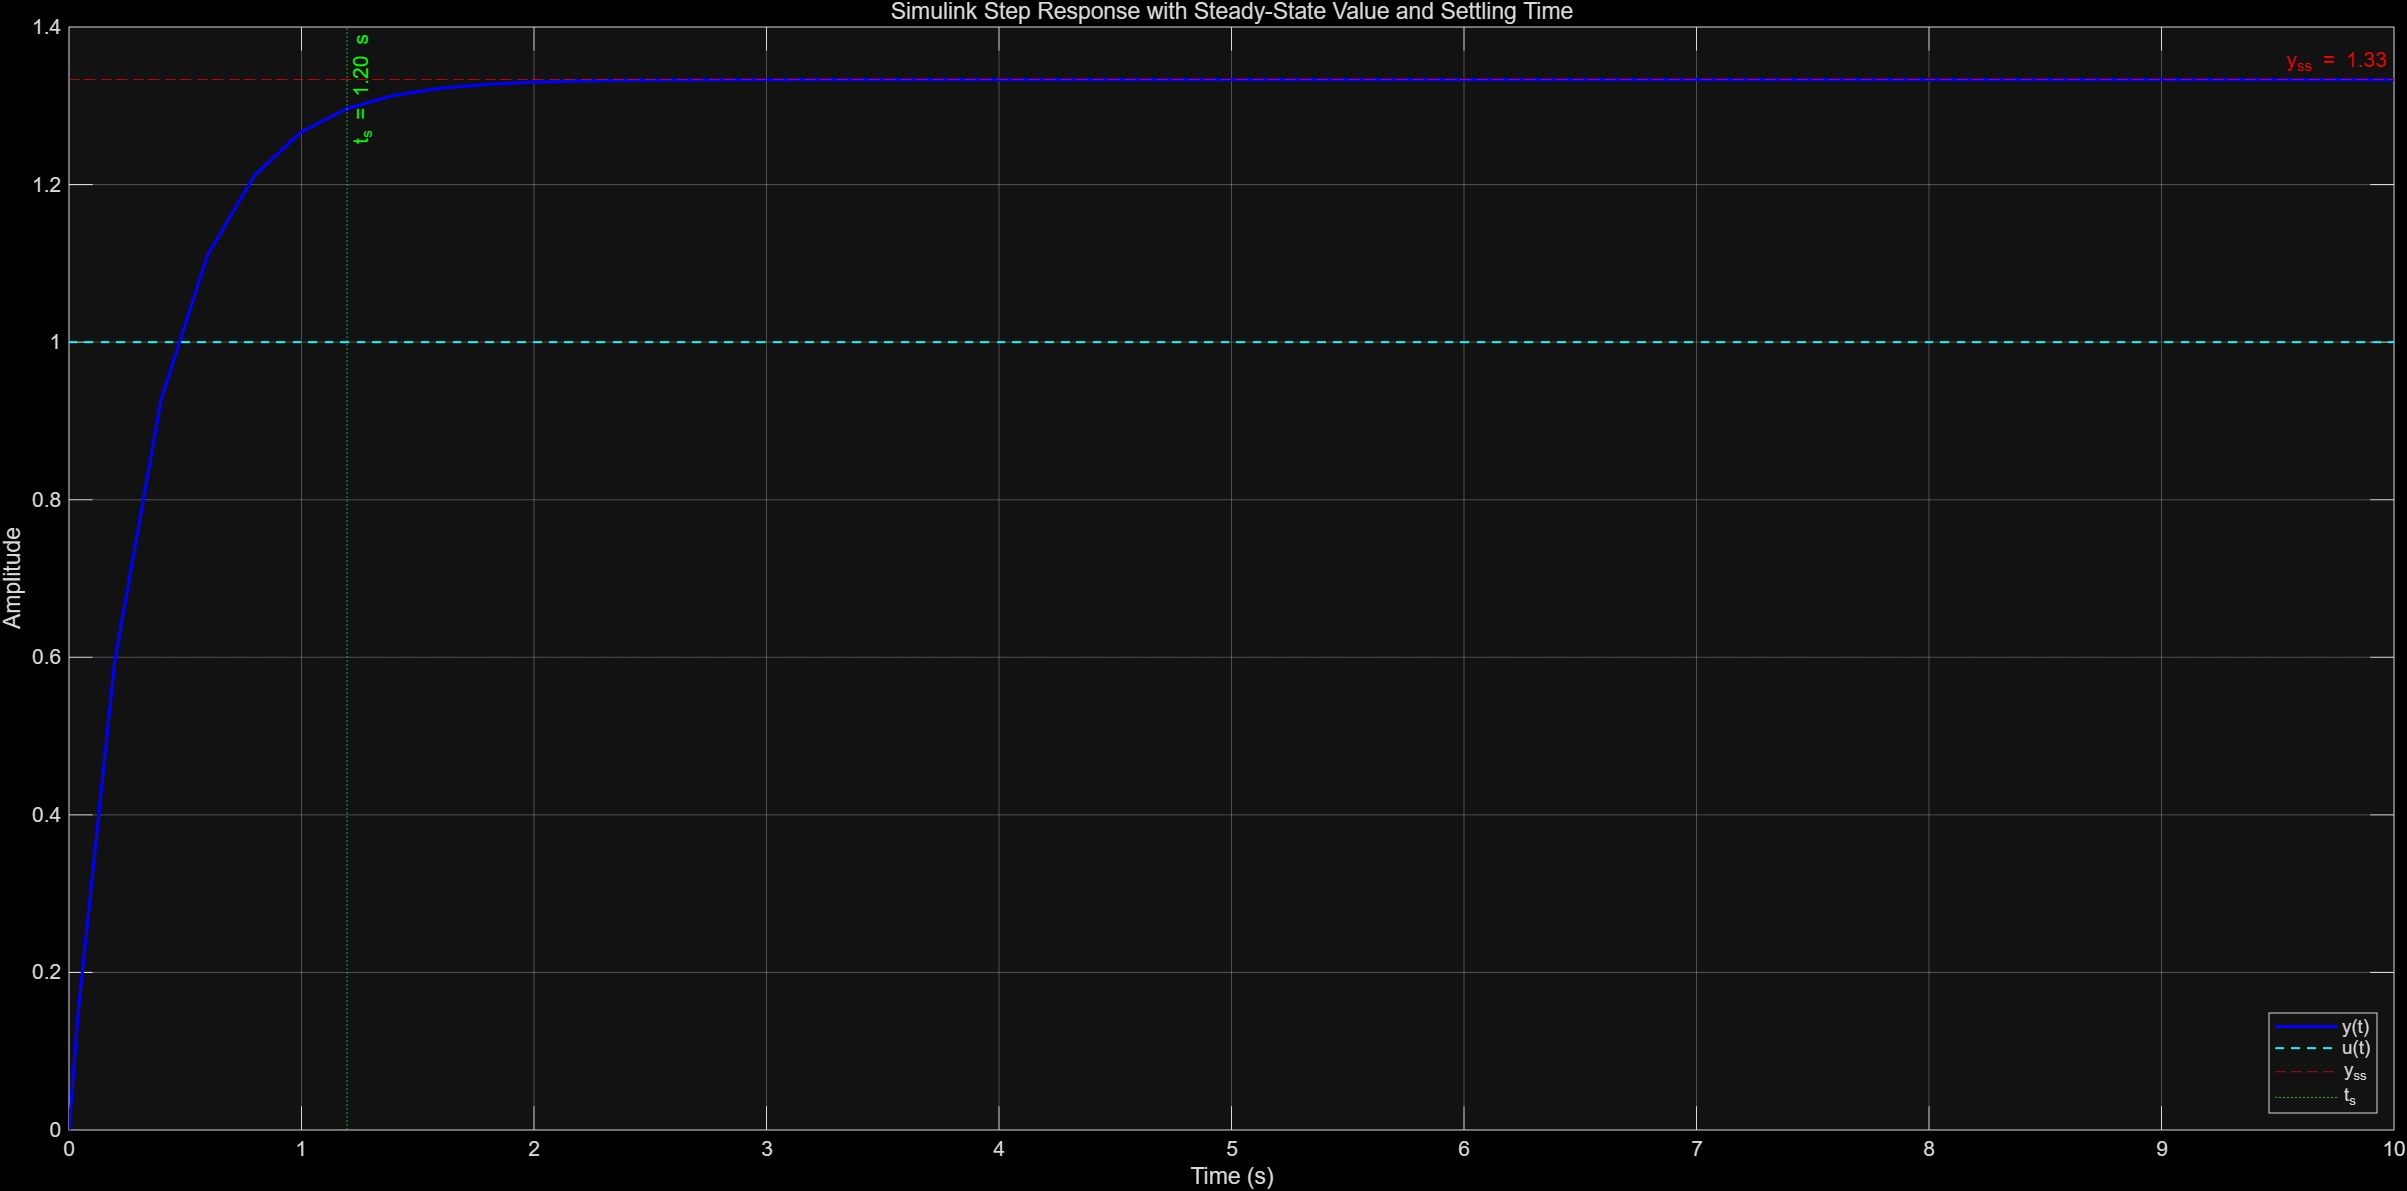
\includegraphics[width=0.6\textwidth]{Q2c.png}
        \end{center}

        \item y(0) = 1:
        \begin{center}
            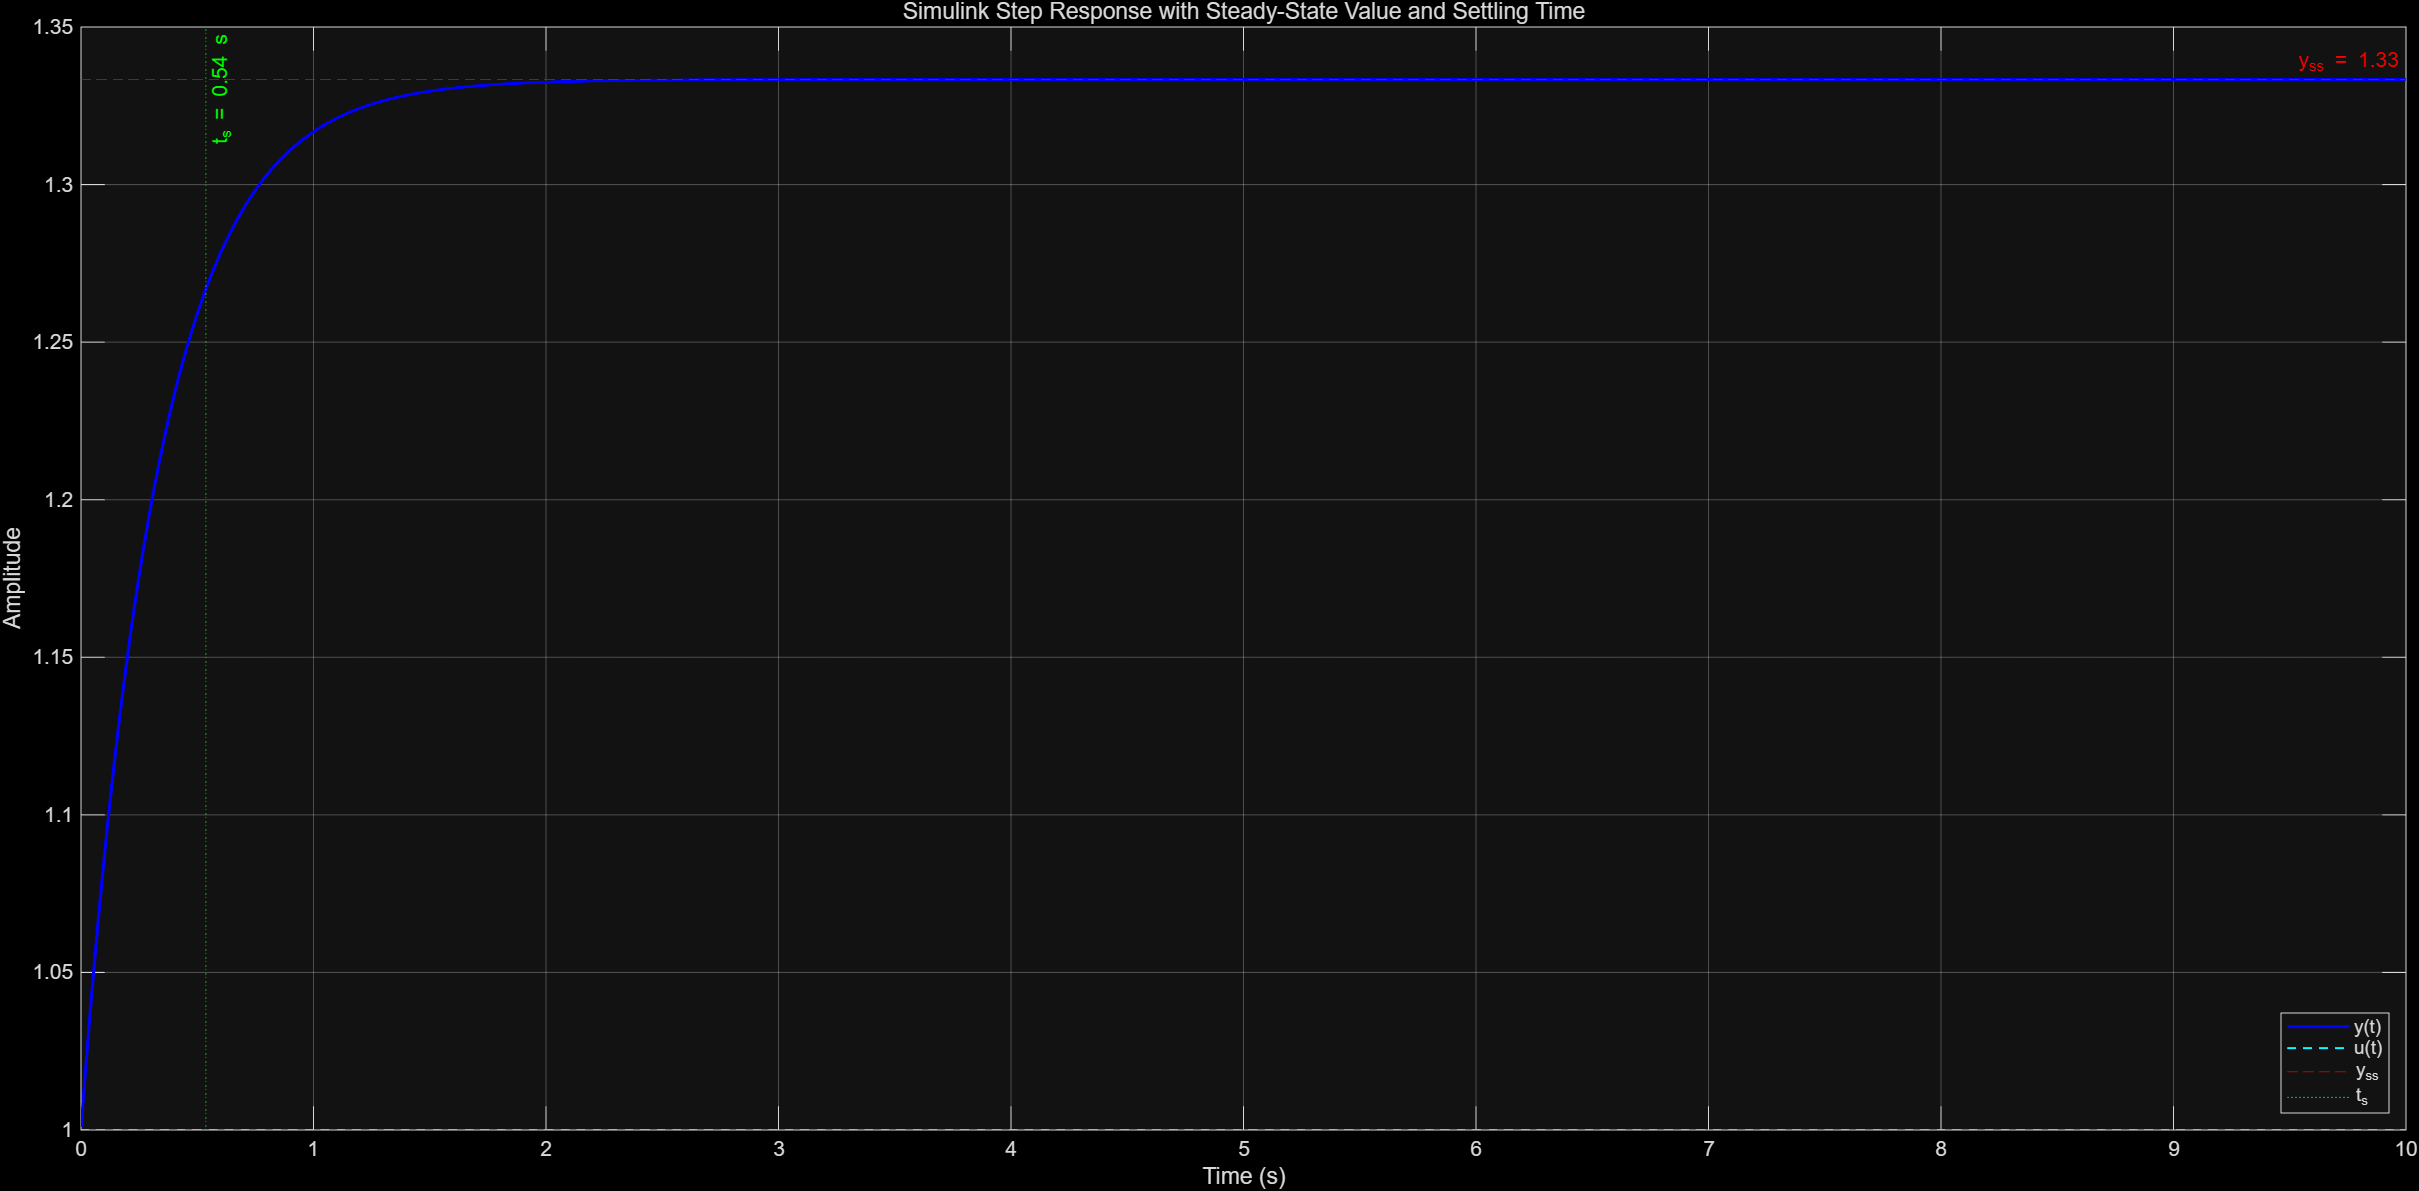
\includegraphics[width=0.6\textwidth]{Q2d.png}
        \end{center}

    \end{enumerate}

\end{document}